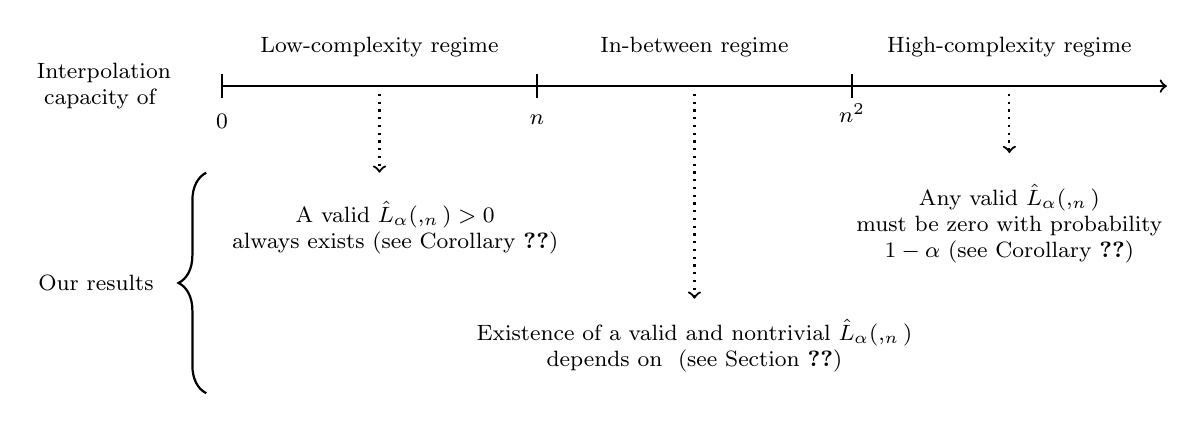
\begin{tikzpicture}

    \tikzstyle{every node}=[font=\footnotesize]

    \draw[thick, ->] (0,0) -- (12, 0);
    \draw[thick] (0, -0.15) -- (0, 0.15) node[anchor=north, yshift = -10.8] {$0$};
    \draw[thick] (4, -0.15) -- (4, 0.15) node[anchor=north, yshift = -10.8] {$n$};
    \draw[thick] (8, -0.15) -- (8, 0.15) node[anchor=north, yshift = -7] {$n^2$};

    
    \node[align = center] at (2,.5) {Low-complexity regime};
    \node[align = center] at (6,.5) {In-between regime};
    \node[align = center] at (10,.5) {High-complexity regime};

    \draw[thick, ->, dotted] (2,-0.1) -- (2,-1.1);
    \node[align = center] at (2.2, -1.8) {A valid $\hat{L}_\alpha(\Fcal,\Dcal_n)>0$\\always exists (see Corollary~\ref{cor:low_complexity_interpolation_capacity})};

    \draw[thick, ->, dotted] (6,-0.1) -- (6,-2.7);
    \node[align = center] at (6, -3.3) {Existence of a valid and nontrivial $\hat{L}_\alpha(\Fcal,\Dcal_n)$ \\ depends on $\Fcal$ (see Section~\ref{sec:boundary})};
    
    \draw[thick, ->, dotted] (10,-0.1) -- (10,-0.85);
    \node[align = center] at (10, -1.75) {Any valid $\hat{L}_\alpha(\Fcal,\Dcal_n)$\\must be zero with probability\\$\gtrapprox 1-\alpha$ (see Corollary~\ref{cor:high_complexity_interpolation_capacity})};

    \node[align = center] at (-1.5, 0) {Interpolation\\capacity of $\Fcal$};

    \node[align = center] at (-1.6, -2.5) {Our results};
    \draw [decorate,decoration={brace,amplitude=10pt}, thick, rotate=90](-3.9, 0.2) -- (-1.1, 0.2);

\end{tikzpicture}